% ******************************* Thesis Appendix C ********************************

\chapter{Ejecuci\'on de RAUFlow}
\label{appendix5}

% **************************** Define Graphics Path **************************
\ifpdf
    \graphicspath{{Appendix5/Figs/Raster/}{Appendix5/Figs/PDF/}{Appendix5/Figs/}}
\else
    \graphicspath{{Appendix5/Figs/Vector/}{Appendix5/Figs/}}
\fi

En el presente anexo se incluyen una guía para la ejecuci\'on de la aplicaci\'on RAUFlow y una descripción de la interfaz web.\\

Para ejecutar la aplicaci\'on es necesario iniciar el controlador Ryu y ejecutar las cuatro aplicaciones Ryu incluidas en la arquitectura. Para ello se ejecuta el siguiente comando en el directorio Proyecto/ryu-master dentro de la estructura de directorios del proyecto.

\begin{center}
\texttt{./bin/ryu run --observe-links ryu/app/proyecto/businessLogic/RAUFlowApp.py}
\end{center}

\begin{figure}[h] 
\centering    
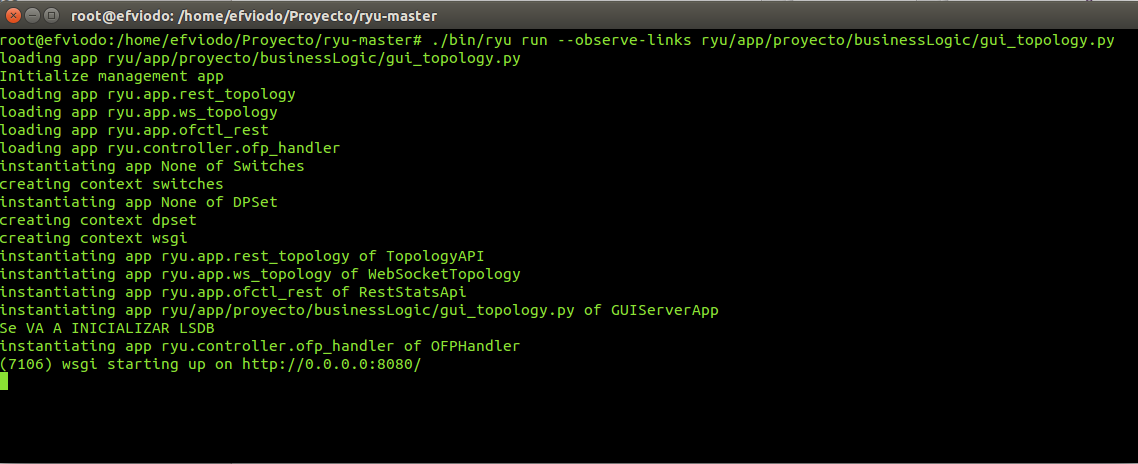
\includegraphics[width=1.0\textwidth]{Snap10}
\caption[Ejecuci\'on RAUFlow]{Ejecuci\'on RAUFlow}
\label{fig:Img2}
\end{figure}

Este comando levanta el controlador Ryu y le pasa como parámetro la aplicaci\'on RAUFlowApp la cual internamente instancia las otras tres aplicaciones Ryu.

Por otro lado la aplicaci\'on instancia la API REST de servicios, por defecto en el puerto 8080 en la direcci\'on localhost. Ambos valores pueden configurarse desde el archivo wsgi.py.\\

Para acceder a la aplicaci\'on abrir desde un navegador web la siguiente direcci\'on:

\begin{center}
http://localhost:8080/
\end{center}


\begin{figure}[ht!] 
\centering    
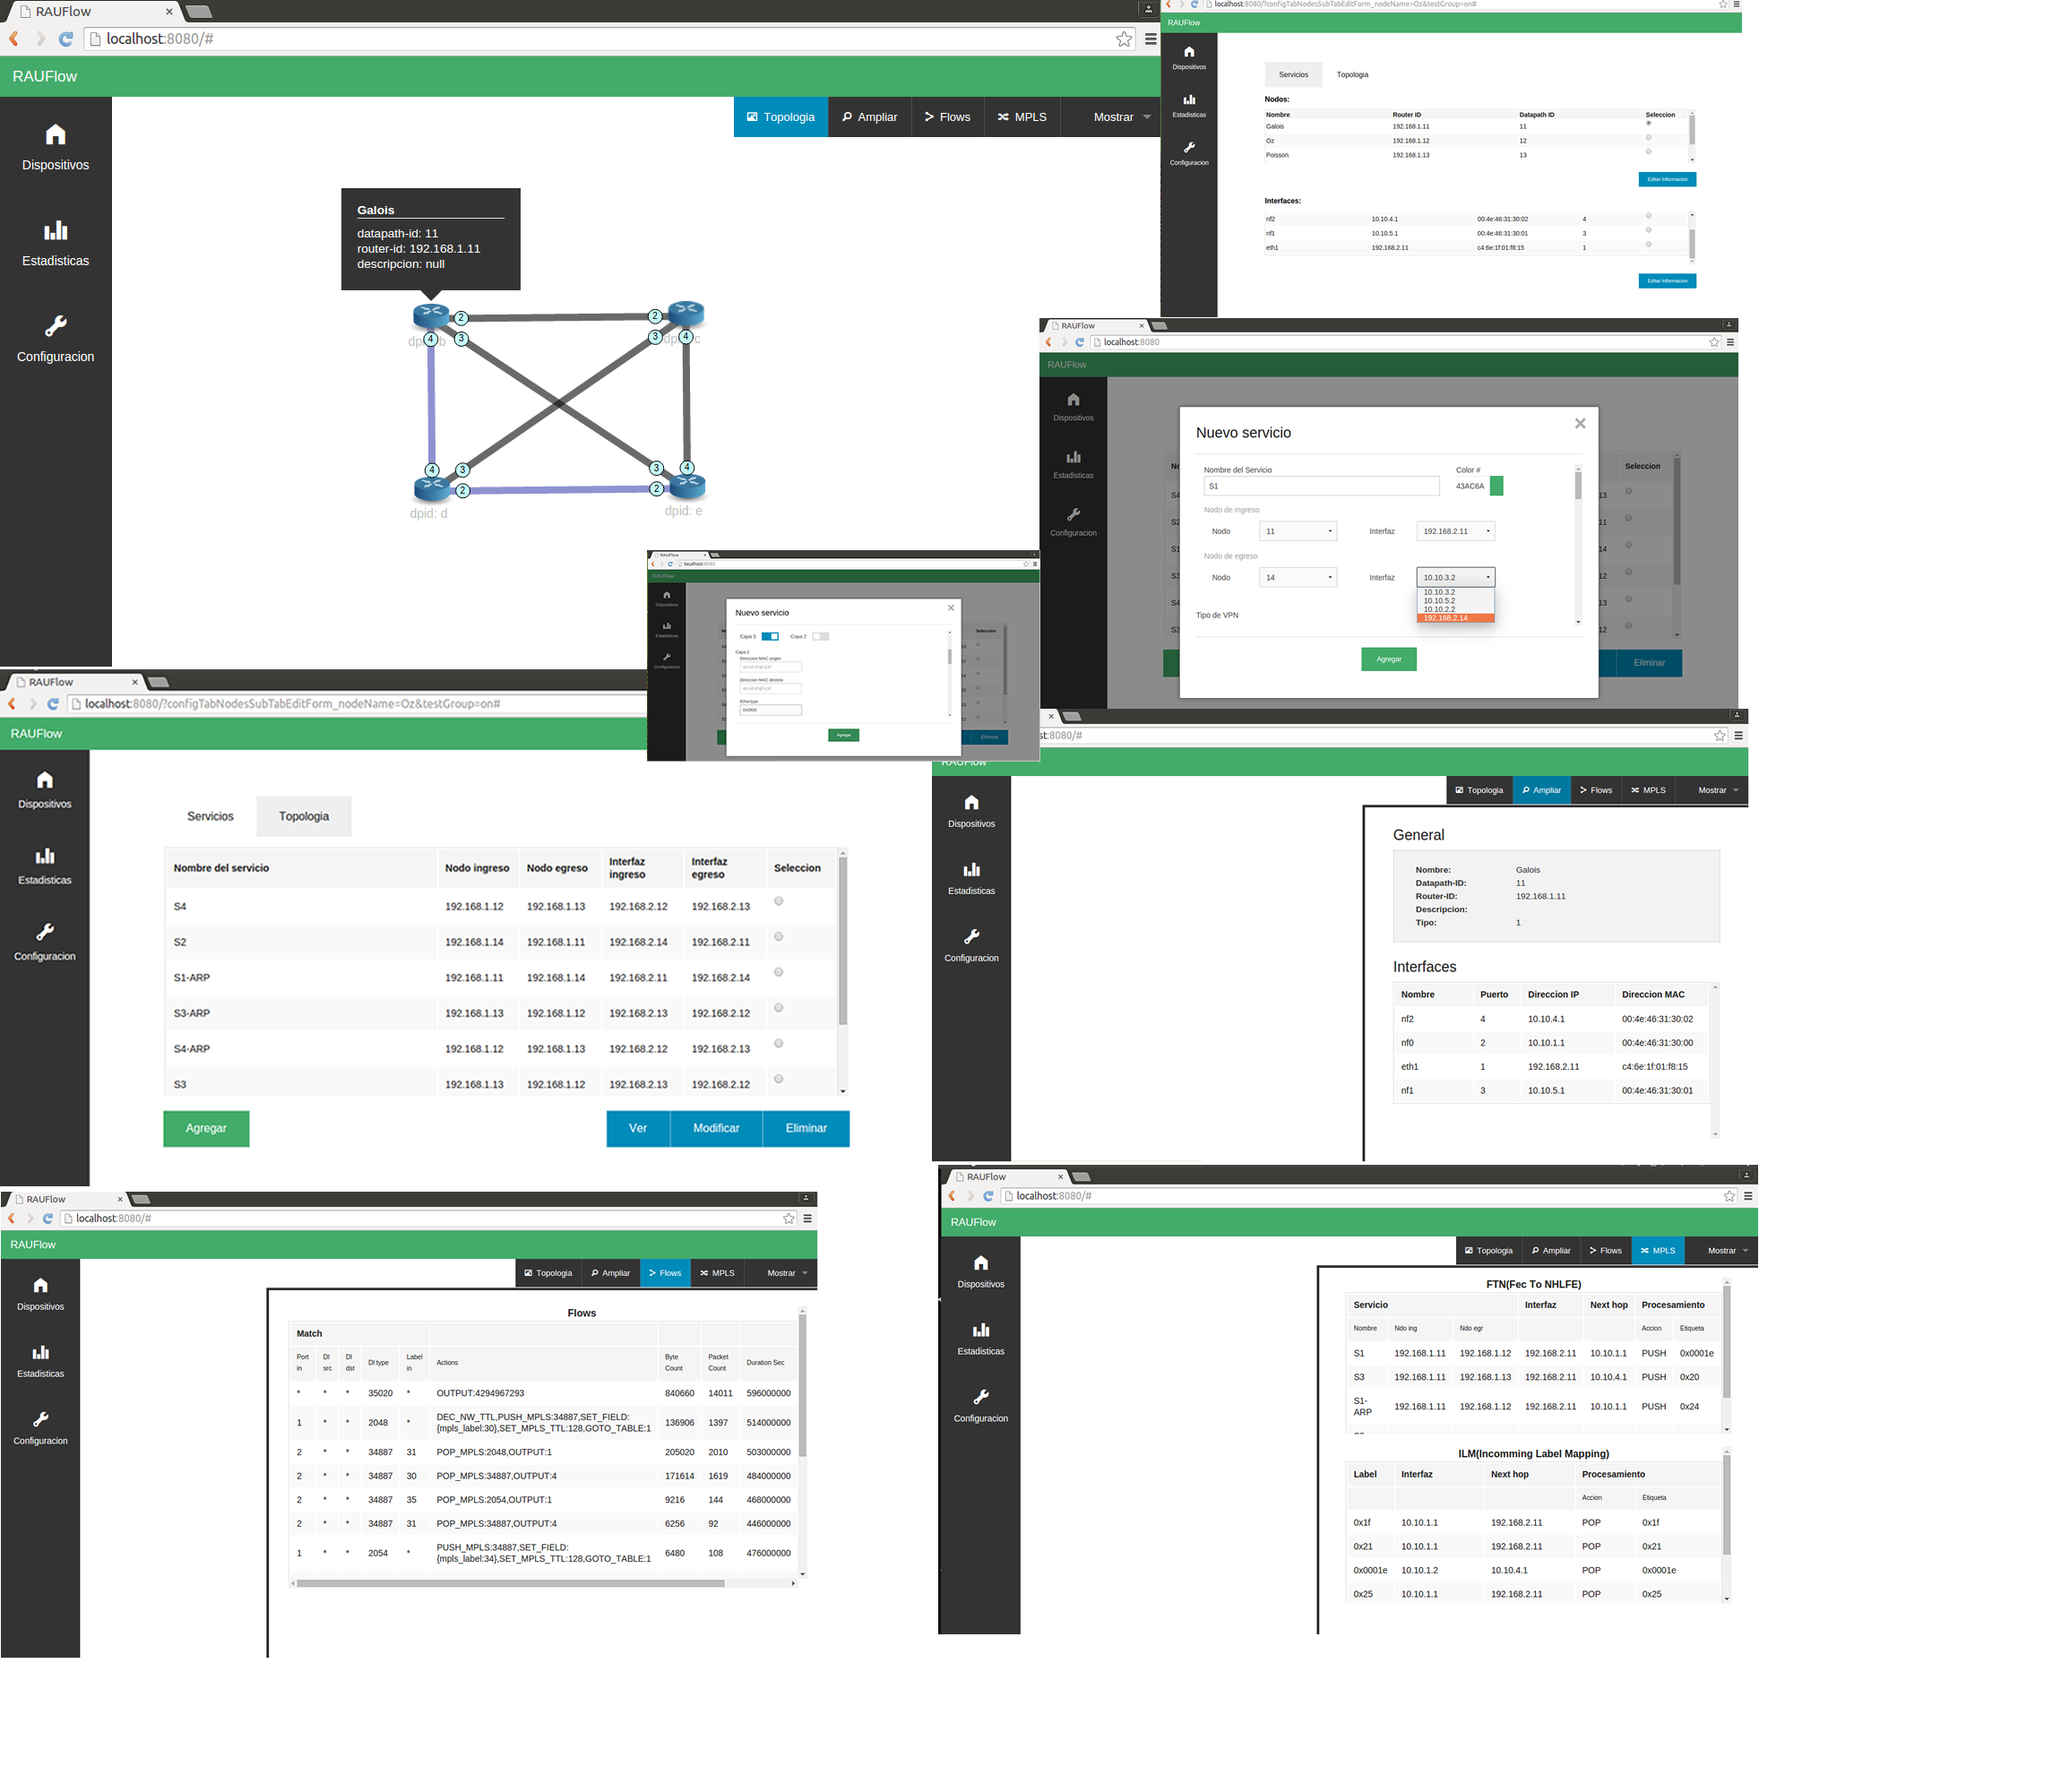
\includegraphics[width=1.2\textwidth]{SnapApp}
\caption[Capturas de interfaz gráfica de RAUFlow]{Capturas de interfaz gráfica de RAUFlow}
\label{fig:Img2}
\end{figure}